\documentclass[12pt]{scrreprt}

% satz nach der norm auf der tu-seite

% \documentclass[12pt,a4paper]{report}
% satzspiegel festlegen
%\usepackage{geometry}
%\geometry{
%  left=4cm,
%  right=1.5cm,
%  top=3cm,
%  bottom=3cm,
%  bindingoffset=0mm
%}

% referenzen
\usepackage{cite}
\usepackage{bibgerm}

% farben definieren
\usepackage{xcolor}
\definecolor{lightblue}{cmyk}{0.346, 0.114, 0, 0.106}


% zeilenabstand (nach dem dokument auf der tu-seite)
\usepackage[onehalfspacing]{setspace}

% deutsch
\usepackage{ucs}
\usepackage[utf8x]{inputenc}
\usepackage[T1]{fontenc}
\usepackage[ngerman]{babel}

% mathe pakete
\usepackage{amsmath,amssymb,amstext}

% einfach bilder einbinden
\usepackage{graphicx}

% fußnoten immer am ende
\usepackage[bottom]{footmisc}

% tabellen
\usepackage[margin=10pt,labelfont=bf]{caption} %abstand zwischen caption und tabelle und fette caption nummer

% codeblöcke
\usepackage{listings}

% abkürzungen
\usepackage[printonlyused]{acronym}

% bessere listen
\usepackage{enumitem}
\setlist{noitemsep} % entfernen der abstände zwischen den verschiedenen items (naja so halb der rest kommt vom zeilenabstand)

% bessere links (sollte als letztes paket geladen werden)
\usepackage[colorlinks=false]{hyperref}



\titlehead{Technische Universität Berlin\\Fakultät IV (Elektrotechnik und Informatik)\\Institut für Softwaretechnik und Theoretische Informatik\\Fachgebiet Übersetzerbau und Programmiersprachen\\Franklinstr. 28/29\\10587 Berlin}
\subject{Diplomarbeit}
\title{Integration von funktionalen Web-Client- und Server-Sprachen am Beispiel von SL und Scala}
\author{Tom Landvoigt, Matrikelnummer: 222115}
\publishers
{
  \begin{tabular}{ll}
    Prüfer:   & Prof. Dr. Peter Pepper\\
              & Prof. Dr.-Ing. Stefan Jähnichen\\
    Betreuer: & Martin Zuber\\
              & Christoph Höger\\
  \end{tabular}
}
\date{\today{}, Berlin}

% DOCUMENT BEGIN 
\begin{document}
\pagenumbering{roman}
\maketitle
\tableofcontents   % Inhaltsverzeichnis
\listoffigures     % Abbildungsverzeichnis
\listoftables      % Tabellenverzeichnis
\lstlistoflistings % Listingverzeichnis
\newpage
\thispagestyle{empty}		% ohne Kopf und Fußzeilen
\begin{LARGE}
	\textbf{Erklärung}
\end{LARGE}

\vspace{1cm}

Hiermit erkläre ich, dass ich die vorliegende Arbeit selbstständig und eigenhändig sowie ohne unerlaubte fremde Hilfe und ausschließlich unter Verwendung der aufgeführten Quellen und Hilfsmittel angefertigt habe.
\vspace{2cm}

Berlin, den \today

\vspace{1cm}
%\rule{_Breite_}{_Stärke_}		%andersrum ist's vertikal

\rule{0.3\textwidth}{0.4pt}

Unterschrift

%\Datum
\vspace*{6cm}
\newpage

\pagenumbering{arabic}

% set style for code blocks
\lstset{basicstyle=\ttfamily\small, numbers=left, numberstyle=\tiny}

\section{Einleitung}

Das World Wide Web ist ein integraler Bestandteil unseres Lebens geworden. Ein Großteil der Software mit der wir in Berührung kommen, benutzt Webseiten als Frontend. Deshalb muss sich jede moderne Programmiersprache daran messen lassen wie leicht es ist mit ihr Webprojekte zu erstellen. Daher bieten Java, Scala, Ruby und viele andere Programmiersprachen Frameworks an um schnell und einfach strukturierte Webprojekte zu erstellen. Ein gemeinsames Problem dieser Frameworks ist es, insbesondere mit dem aufkommen von Rich Internet Applications, das clientseitig Code ausgeführt werden muss. In diesem Bereich hat sich \ac{JS} zum Quasistandard entwickelt\footnote{Es gibt weitere Alternativen wie Java oder Flash, die aber Browserplugins vorraussetzen.}. Dadurch ist man beim Schreiben von browserseitigen Funktionen auf die von den \ac{JS}-Entwicklern bevorzugten Programmierparadigmen wie dynamische Typisierung festgelegt. Bei größeren Bibliotheken kann dies die Wartung und Weiterentwicklung erschweren.

Im Rahmen eines Projekts \cite{Buchle2013} an der TU-Berlin wurde die typsichere funktionale Sprache \ac{SL} entwickelt die nach \ac{JS} compiliert. Andererseits wurde Mitte 2013 durch die Einführung von compiler makros \cite{Burmako2013} die Metaprogrammierung innerhalb von Scala erheblich vereinfacht.

Im Rahmen eines Papers \cite{Hoger2013} wurde gezeigt, das es möglich ist mit Hilfe von Compilermakros statischen \ac{SL} Code inline in Scala zu benutzen. Dazu wurde eine Beispielanwendung im Play Framework geschrieben \cite{Play1}. Diese Einbettung sollte im Zuge dieser Diplomarbeit erweitert werden. Es ist nun möglich Scala Funktionen und Werte in einem gewissen Rahmen automatisch zu übersetzen und typsicher im \ac{SL} Code zu benutzen.

Für das Verständnis der Diplomarbeit werden Kenntnisse im Bereich funktionaler Programmierung sowie Grundlagen in den Sprachen Scala und \ac{JS} vorausgesetzt.

\chapter{ Einführung in Simple Language}

Mitte 2013 wurde \ac{SL} als einfache funktionale Lehrsprache für den Studienbetrieb der TU-Berlin entwickelt. Im Rahmen des Compilerbauprojekts im Sommersemerster 2013 wurde \ac{SL} von den Studierenden um die Möglichkeit der Modularisierung erweitert \cite{Bisping2013}. \ac{SL} ist eine strikt getypte funktionale Sprache.

Ein \ac{SL} Programm besteht aus einer Menge von Modulen. Ein Modul ist eine Textdatei mit der Endung '.sl'. In ihm können Funktionen und Typen definiert werden. Durch die Übersetzung eines \ac{SL} Moduls werden zwei Dateien erzeugt. Die Datei mit der Endung '.ls.js' enthält den ausführbaren JavaScript-Code. Die zweite Datei mit der Endung '.signature' enthält Informationen darüber welche Funktionen und Datentypen in anderen Modulen verwendet werden können. Das Modul prelude.sl beschreibt alle vordefinierten Funktionen und Datentypen und wird in alle Programme eingebunden. 

Der Syntax soll hier nur Beispielhaft beschrieben werden.

\begin{lstlisting}[caption=Beispielmodul, label=lst:bsp1]
-- Kommentar

IMPORT "std/basicweb" AS Web [1.]
IMPORT EXTERN "foo/_bar"

DATA StringOrOther a = Nothing | StringVal String | OtherVal a [4.]

PUBLIC FUN getOtherOrElse : StringOrOther a -> a -> a [2.]
DEF getString (OtherVal x) y = x
DEF getString x y = y

PUBLIC FUN main : DOM Void [3.]
DEF main = Web.alert(intToString (getOtherOrElse(exampleVar, 3)))

FUN exampleVar : StringOrOther Int
DEF exampleVar = OtherVal 5

FUN getDocumentHight : DOM Int
DEF getDocumentHight = {| window.outerHeight |} : DOM Int

\end{lstlisting}

\begin{enumerate}
  \item Mit \lstinline!IMPORT "<Pfad>" AS <Bezeichner>! können Module nachgeladen werden. Typen und Funktionen die aus Fremdmodulen benutzt werden müssen mit dem \lstinline!<Bezeichner>! qualifiziert werden. Ein Beispiel dafür ist \lstinline!Web.alert(...)!. 
  
  Mit \lstinline!IMPORT EXTERN! können \ac{JS}-Quelldateien eingebunden werden. In diesem Fall würde der Inhalt der Datei \lstinline!\_bar.js! im Ordner \lstinline!foo! an den Anfang des Kompilats kopiert werden.
  \item Die optionale Typdefinition einer Funktion kann mit \lstinline!FUN <Funktionsname> : <Typ>! angegeben werden. Wenn ein \lstinline!PUBLIC! vorgestellt wird, ist die Funktion auch außerhalb des Moduls sichtbar. Darauf folgen eine oder mehrere pattern basierte Funktionsdefinition der Form \lstinline!DEF <Funktionsname> = <Funktionsrumpf>!.
  \item Ein Spezialfall bildet die Funktion \lstinline!main!. Sie bildet den Einstiegspunkt in ein \ac{SL} Programm. Sie hat den festen Typ \lstinline!DOM Void!. \lstinline!DOM a! und \lstinline!Void! sind einige der Vordefinierten Typen. \lstinline!Void! bezeichnet den leeren Typen, also keinen Rückgabewert. \lstinline!DOM a! ist der Typ der \ac{JS}-quoating Monade. Mit ihr können \ac{JS} Snippets in \ac{SL} eingebunden werden (Beispiel: \lstinline!{| window.outerHeight |} : DOM Int!). Weiter vordefinierte Typen sind \lstinline!Char! und \lstinline!String! um Zeichen(ketten) darzustellen, sowie \lstinline!Int! für ganzzahlige Werte und \lstinline!Real! für Gleitkommazahlen. Der letzte vordefinierte Typ ist \lstinline!Bool! für boolesche Werte.
  \item Mit \lstinline!DATA <Typname> [<Typprameter> ...] = <Konstruktor> [<Typparameter> ...] | ...! können eigene Typen definiert werden. Wie wir Scala Typen und Werte nach \ac{SL} und zurück übersetzen wird Stoff des nächsten Kapitels (\ref{cha:model-sharing}) sein.
\end{enumerate}

\ac{SL} bietet noch weitere Eigenschaften wie Lambdafunktionen, benutzerdefinierte Operatoren und 'LET IN'-Ausdrücke, diese sind aber nicht für das Verständnis der Diplomarbeit relevant. Bei Interesse kann eine vollständige Beschreibung der Sprache im Report des Compilerbauprojekts \cite{Bisping2013} nachgelesen werden.

\chapter{Model Sharing}
\label{cha:model-sharing}

Im Zuge dieser Arbeit sollten Scala-Werte und -Funktionen in \ac{SL} eingebettet werden. Dazu muss einem Scala Typ ein \ac{SL} Typ zugeordnet werden. Betrachten wir dazu die Scala Funktion \lstinline!foo! im Listing \ref{lst:scala-fun-example}.

\begin{lstlisting}[caption=Beispielfunktion foo, label=lst:scala-fun-example]
def foo( i: Float ): Double = {...}
\end{lstlisting}

Für die Typen \lstinline!Float! und \lstinline!Double! müssen wir ihre \ac{SL}-Entsprechung finden. Um die Implementation zu vereinfachen setzen wir voraus, das jedem Scala Typ genau ein \ac{SL}-Typ zugeordnet wird. Andernfalls müssten wir für alle möglichen Permutationen einen \ac{SL}-Funktionsrumpf erstellen. Bei eingebetteten Scala Werten müsste der SL-Code analysiert werden, um die passende Übersetzung zu finden\footnote{Das ist keine besonders große Einschränkung, da wie wir später sehen werden, das das Typsystem von SL sehr einfach ist und dadurch viele Scala-Typen auf ein und den selben SL Typen abgebildet werden. }. Wir erhalten die partielle Funktion $translate_{type}(Type_{Scala}) = Type_{SL}$. Diese wird in Abschnitt \ref{subsec:translate_type} behandelt.

Haben wir einen passenden Typen gefunden, müssen auch die Werte in einander überführt werden. Dies sollte eine bijektive Abbildung sein. Das dies nicht immer möglich ist, wird in Abschnitt \ref{sec:value-transformation} behandelt.

Für \lstinline!Float! und \lstinline!Double! ist der SL Typ \lstinline!Real! die semantisch beste Wahl. Im Ergebnis erhalten wir schematisch die Funktion \lstinline!sl_foo! aus Listing \ref{lst:scala-fun-example-translate}.

\begin{lstlisting}[caption=Übersetzung von foo, label=lst:scala-fun-example-translate]
FUN sl_foo : Real -> Real
DEF sl_foo p0 = double_to_real (call_via_ajax (foo (real_to_float p0) ) )
\end{lstlisting}

\section{Typübersetzung}
\label{sec:type-translation}

In den nächsten Abschnitten wird die Typübersetzung betrachtet. Also welche Scala Typen mit welchen SL Typen assoziiert werden. Dazu werden die beiden Typsysteme kurz erläutert und dann die Funktion $translate_{type}$ näher beschrieben.

\subsection{SL Typsystem}

Das Typsystem von \ac{SL} ist (entsprechend seines Anspruches als Lehrsprache) sehr einfach. Es gibt eine Reihe von vordefinierten Typen \lstinline!Int!, \lstinline!Real!, \lstinline!Char!, \lstinline!String!, \lstinline!Bool! und \lstinline!Void! sowie den Typ der \ac{JS}-Quoting Monade \lstinline!DOM a!\footnote{Typen werden groß geschrieben, Typvariablen klein. \lstinline!DOM a! steht also zum Beispiel für \lstinline!DOM Void!, \lstinline!DOM Int! usw.}. Mit dem Stichwort \lstinline!DATA! können eigene Konstruktor-/Summentypen definiert werden \cite[S. 123]{Pepper2007}.

\begin{lstlisting}[caption=Beispiele für selbst definierte Datentypen in \ac{SL}, label=lst:bsp2]
-- Summentyp
DATA Fruits = Apple | Orange | Plum

-- Konstruktortyp
DATA CycleKonst = Cycle Int Int

-- Mischung aus Konstruktor- und Summentyp mit Typvariablen
DATA Either a b = Left a | Right b
\end{lstlisting}

\subsection{Scala Typsystem}

Das Scala Typsystem in Gänze zu erklären würde den Rahmen dieser Arbeit bei weitem sprengen \cite{Odersky2013}. Im Rahmen dieser Arbeit wurden nur einige wenige vordefinierte Typen übersetzt.

Scala ist strikt Objektorientiert. Es kennt keine primitiven Typen. Alle Typen sind Objekte, aber es gibt vordefinierte Objekttypen die den primitiven Datentypen von Java zugeordnet werden können \cite{Paggen2013}. Im Folgenden werden die Typen \lstinline!Byte!, \lstinline!Short!, \lstinline!Int!, \lstinline!Long!, \lstinline!Float!, \lstinline!Double!, \lstinline!Boolean!, \lstinline!Char!, \lstinline!String! und \lstinline!Unit! trotzdem als die primitiven Typen von Scala bezeichnet. Die Vererbungshierarchie einiger vordefinierter Objekttypen kann dem Bild \ref{fig:classhierarchy} entnommen werden.

\begin{figure}[h] 
  \centering
     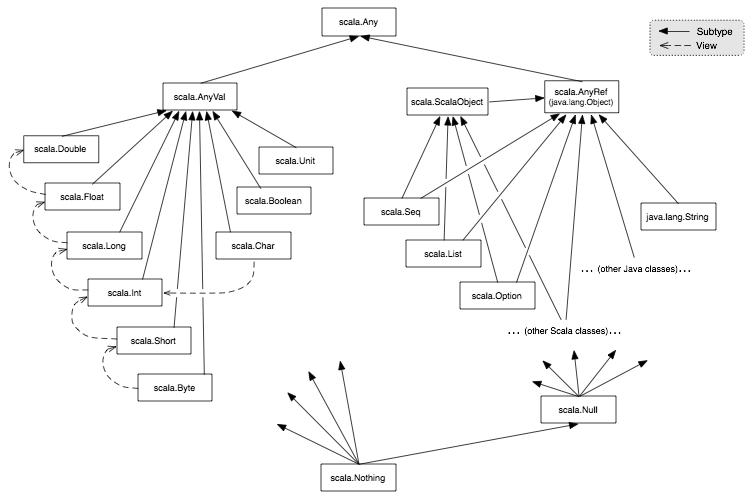
\includegraphics[width=\textwidth]{Bilder/classhierarchy}
  \caption{Vererbungshierarchie einiger Scala Klassen \cite{UnbekannterAutor2013}}
  \label{fig:classhierarchy}
\end{figure}

Es gibt in Scala, Konstrukte, die den selbst definierten Typen aus \ac{SL} sehr ähnlich sind. Das wird anschaulich am Beispiel von Option (siehe Listing \ref{lst:option-in-sl-scala}). Es wurden aber auch andere vordefinierte Typen wie \lstinline!Seq[A]! übersetzt, deren innere Struktur sich stark von ihrem SL Äquivalent \lstinline!List a! unterscheiden.

\begin{lstlisting}[caption=Option in \ac{SL} und Scala, label=lst:option-in-sl-scala, float=h]
Option in SL:
PUBLIC DATA Option a = Some a | None

Option in Scala:
sealed abstract class Option[+A] ... { ... }

final case class Some[+A](x: A) extends Option[A] { ... }

case object None extends Option[Nothing] { ... }
\end{lstlisting}

\subsection{Funktion $translate_{type}$}
\label{subsec:translate_type}

Bei der Wahl eines SL Partnertyps für einen Scala Typ sollte auf zwei Bedingungen geachtet werden:

\begin{enumerate}
 \item{Die Typen sollten semantisch ähnlich sein.}
 \item{Es sollte eine semantisch sinnvolle bijektive Abbildung zwischen den Werten der beiden Typen existieren. }
\end{enumerate}

Wie wir im Abschnitt \ref{sec:value-transformation} sehen werden, wird die zweite Bedingung für einige primitiven Datentypen von Scala verletzt. Insbesondere für die ganzzahligen Primitiven kann sie nicht eingehalten werden. Da dadurch eine entsprechende Fehlerbehandlung unumgänglich wurde und um die Bedienung zu erleichtern wurden die Fließkommaprimitiven mit \lstinline!Real! und die ganzzahligen Primitiven mit \lstinline!Int! assoziiert.


\begin{table}[h]
\caption{Die Funktion $translate_{type}$}
\centering
\begin{tabular}{ll|ll}
Scala Typ & \ac{SL} Typ & Scala Typ & \ac{SL} Typ \\
\hline
\\
Float     & Real        & Char      & Char \\
Double    & \\
          &             &           & \\
Byte      & Int         & Boolean   & Bool \\
Short     & \\
Int       &             & Unit      &  Void \\
Long      & \\
          &             &           & \\
String    & String \\
          &             &           & \\
Seq[A]    & List a      & Option[A] & Option a

\end{tabular}
\label{tab:translate_type}
\end{table}

Bei generischen Datentypen wie \lstinline!Seq[A]! folgt aus den oben genannten Bedingungen, das die Anzahl der Typparameter der Partnertypen gleich sein sollte. Wenn ein generischer Datentyp übersetzt werden soll, wird versucht die Typparameter rekursiv zu übersetzen. Ist dies möglich kann auch der gesamte Typ übersetzt werden. Also \lstinline!Seq[Option[Long]]! würde zu \lstinline!List Option Int! übersetzt werden. Eine vollständige Auflistung von $translate_{type}$ findet sich in Tabelle \ref{tab:translate_type}.

\section{Darstellungsübersetzung}
\label{sec:value-transformation}

Wie bereits in der Einführung dieses Kapitels erwähnt, wählen wir die Wertübersetzungsfunktionen anhand des Scala Typs. Da \ac{SL} nach \ac{JS} kompiliert muss ein Scala Wert entsprechend seines Typs in eine passende \ac{JS} Darstellung übersetzt werden. Für die Gegenrichtung, also \ac{SL} nach Scala gilt dies analog. 

\subsection{Übersetzung von primitiven Werten}

Vor allem bei der Übersetzung von Primitiven existiert das Problem der unterschiedlichen Wertebereiche. Man kann zwar jeden Wert des Scala Typs \lstinline!Byte! in einen Wert des \ac{SL} Typs \lstinline!Int! übersetzen, aber nicht umgekehrt. In der Tabelle \ref{tab:primitives-borders} werden die Wertebereiche für primitive Typen aufgelistet. Kann ein Wert von einer Darstellungsform nicht in die andere Darstellungsform umgewandelt werden muss dieser Fehler behandelt werden (siehe Abschnitt \ref{sec:trans-implementation}). 

Bei den ganzzahligen Primitiven fällt auf, das für den Wertebereich gilt:
\begin{center}
$|$\lstinline!Int!$| < |$\lstinline!Number!$| < |$\lstinline!Long!$|$
\end{center}

\begin{table}
\caption{Umfang der primitiven Datentypen in Scala und \ac{SL} (\ac{JS})\cite[S. 28-30]{Ecma2011}\cite{Oracle2011}}
\centering
\begin{tabular}{lll}
 \ac{SL} &    \ac{JS} Darstellung              &    Scala \\
\\
Int  &  Number\footnotemark $[-2^{53} + 1, 2^{53} -1]$   &  Byte  $[-128, 127]$\\
Int  &  Number $[-2^{53} + 1, 2^{53} -1]$   &  Short $[-2^{15}, 2^{15}-1]$\\
Int  & Number $[-2^{53} + 1, 2^{53} -1]$    & Int   $[-2^{31}, 2^{31}-1]$\\
Int  &  Number $[-2^{53} + 1, 2^{53} -1]$   &  Long  $[-2^{63}, 2^{63}-1]$\\
\\
Real &  Number (IEEE 754 64-Bit)      &  Float  (IEEE 754 32-Bit)\\
Real &  Number (IEEE 754 64-Bit)      &  Double (IEEE 754 64-Bit)\\
\\
Bool &  Boolean ${true, false}$         &  Boolean ${true, false}$\\
\\
Char &  String (Länge 1) (16-Bit)     &  Char (16-Bit)\\
\\
String& String\footnotemark (maximale Länge: ?)    &  String (maximale Länge: ?)\\
\end{tabular}
\label{tab:primitives-borders}
\end{table}
\footnotetext[6]{Alle Zahlendatentypen werden in \ac{JS} durch den primitiven Number Datentyp dargestellt. Dies ist eine Gleitkommazahldarstellung nach dem IEEE 754 Standard mit einer Breite von 64 Bit. In dieser Darstellung können Ganzzahlwerte von $-2^{53} + 1$ bis $2^{53} -1$ korrekt dargestellt werde.}
\footnotetext{Die maximale Länge von Strings in \ac{JS} und Scala ist Implementationsabhängig.}

\subsection{Übersetzung von komplexen Werten}

Bei nicht primitiven Werten ist mehr Aufwand nötig. Dafür müssen wir zunächst die JS-Darstellung von selbst definierten SL Typen verstehen\footnote{Das beschriebene Schema wurde aus dem SL Compiler generierten Code abgeleitet. Es ist nicht dokumentiert.}.

\begin{lstlisting}[caption=Beispiel eines selbstedefinierten Typs, label=lst:example-datatype-sl]
DATA People a b = Alice | Bob Int | Cesar a b | Octavian
\end{lstlisting}

Die einzelnen Konstruktoren erhalten entsprechend ihrer Reihenfolge eine \lstinline!_cid! beginnend bei $0$. Hat ein Konstruktor keine Parameter, wird er nur durch seine \lstinline!_cid! dargestellt. Andernfalls wird ein Objekt erzeugt. Dies besitzt das Attribut \lstinline!_cid! sowie entsprechend der Anzahl der Parameter Attribute die von \lstinline!_var0! bis \lstinline!_varN! benannt sind. Die JS Darstellung von dem Beispieltyp aus Listing \ref{lst:example-datatype-sl} findet sich in der Tabelle \ref{tab:js-code-of-people}.

\begin{table}[h]
\caption{JS Darstellung des \ac{SL} Typen \lstinline!People Char Bool!}
\centering
\begin{tabular}{ll}
 \ac{SL}              &  \ac{JS} Darstellung \\
\lstinline!Alice!           &  \lstinline!0! \\
\lstinline!Bob 42!          &  \lstinline!{ "_cid" => 1, "_var0" => 42 }! \\
\lstinline!Cesar "a" true!  &  \lstinline!{ "_cid" => 2, "_var0" => "a", "_var1" => true }! \\
\lstinline!Octavian!        &  \lstinline!3! \\
\end{tabular}
\label{tab:js-code-of-people}
\end{table}

An Hand dieses Schemas können wir nun eine Darstellungsübersetzung für den Scala Typ Option (siehe Listing \ref{lst:option-in-sl-scala}) erzeugen:

%Bild: Übersetzung von Option Werten
\begin{table}[h]
\caption{Übersetzung von Option Werten}
\centering
\begin{tabular}{lll}
Scala                   & \ac{JS} Darstellung                        & SL \\

\lstinline!Option[Int]! &                                            & \lstinline!Option Int! \\

\lstinline!Some(15)!    & \lstinline!{ "_cid" => 0, "_var0" => 15 }! & \lstinline!Some(15)! \\
\lstinline!None!        & \lstinline!1!                              &  \lstinline!None! \\
\end{tabular}
\end{table}

%TODO vllt noch Seq[A] zu List a erklären

\section{Erleuterung der Implementation}
\label{sec:trans-implementation}

Die Paare der Funktion $translate_{type}$ werden durch Klassen, die von \lstinline!AbstractTranslator! erben, dargestellt. Sie sind nach dem jeweiligen Scala Typen den sie übersetzen benannt\footnote{zB. \lstinline!SeqTranslator!}. Ihre Hauptfunktion ist \lstinline!translate! (siehe Listing \ref{lst:main-function-translate}). Ihr wird ein Scala Typ übergeben. Wenn der übergebene Scala Typ der Klasse entspricht erhält man als Rückgabewert den entsprechenden \ac{SL} Typen, die Import Statements um die entsprechenden \ac{SL} Module zu laden\footnote{Bei primitiven \ac{SL} Typen sind diese leer. Für den \ac{SL} Typ \lstinline!List.List Opt.Option Int! würde \lstinline!IMPORT "std/option" AS Opt, IMPORT "std/list" AS List! zurück gegeben werden.} sowie die \ac{AST}-Repräsentation der Wertübersetzungsfunktionen von Scala nach \ac{SL} und umgekehrt. Andernfalls wird \lstinline!None! zurückgegeben.

\begin{lstlisting}[caption=Hauptfunktion in AbstractTranslator, label=lst:main-function-translate]
def translate
  ( context: MacroCtxt )
  ( input: context.universe.Type, translators: Seq[AbstractTranslator] )
: Option[( String, 
           Set[String], 
           context.Expr[Any => JValue], 
           context.Expr[JValue => Any] )]
\end{lstlisting}

Weiter Parameter sind \lstinline!context! und \lstinline!translators!. \lstinline!context! ist der Makro Kontext\footnote{siehe Kapitel \ref{chap:scala-compiler-macros}}. Er wird benötigt um \ac{AST}s aufzubauen und den übergebenen Typen zu prüfen. Mit \lstinline!translators! wird der Teil von $translate_{type}$ übergeben mit denen Spezialisierungen eines generischen Typs übersetzt werden können.

Möchte man einen Scala Typ nicht nur gegen eine Klasse prüfen kann man die Hilfsfunktion \lstinline!useTranslators! aus dem companion object von \lstinline!AbstractTranslator! nutzen.


\begin{lstlisting}[caption=Statische Hilfsfunktion in AbstractTranslator, label=lst:hilfsfunktionen]
def useTranslators
  ( context: MacroCtxt )
  ( input: context.universe.Type, translators: Seq[AbstractTranslator] )
: Option[( String,
           Set[String], 
           context.Expr[Any => JValue], 
           context.Expr[JValue => Any] )]
\end{lstlisting}

\lstinline!translators! gibt hier an welchen Teil der Funktion $translate_{type}$ man nutzen möchte\footnote{\lstinline!translators! wird in diesem Fall auch für die Spezialisierungen von generischen Typen benutzt.}. 

Die Wertübersetzungsfunktionen haben die Signatur \lstinline!Any => JValue! bzw. \lstinline!JValue => Any!. \lstinline!JValue! ist Teil der json4s Bibliothek \cite{Json4s}, die benutzt wird um JS Werte zu erzeugen. Insbesondere übernimmt sie in der aktuellen Implementation die Übersetzung der primitiven Werte.

In Anhang \ref{subsec:option-translator} kann eine kommentierte Variante des OptionTranslators eingesehen werden.

\chapter{Scala Compiler Macros}
\label{chap:scala-compiler-macros}

Wie bereits erwähnt wurde, konnte in einem Paper der Technischen Universität Berlin gezeigt, das man mit Hilfe von Compiler Macros statischen \ac{SL} Code in die Views von Play-Anwendungen einbetten kann\cite{Hoger2013}. Mit der Erweiterung von \ac{SL} durch ein Modul-System musste dieses Makro komplett neu geschrieben werden.

Es blieb aber ein grundsätzliches Problem erhalten. Wie kann der generierte \ac{JS}-Code auf das Serverumfeld wie Datenbanken, Session oder Benutzerdaten zugreifen. In herkömmlichen Anwendungen gibt es zwei Lösungen dafür: Entweder man bindet die Daten direkt in den Quellcode der einzelnen Webseite ein oder lädt sie mit Hilfe von Ajax nach. In der aktuellen Version von \ac{SL} kann man Scala-Werte direkt im \ac{SL} Code benutzen und Daten über übersetzte Scala Funktionen nachladen bzw. verändern.

\section{Struktur des Projekts}
\label{sec:project-structure}

Um Scala Funktionen für die Verwendung in \ac{SL}-Code zu markieren wurden die macro annotation \lstinline!sl_function! geschrieben, welche im Abschnitt \ref{sec:annotation-macro} behandelt wird. Im darauf folgenden Abschnitt \ref{sec:inline-macro} wird beschrieben, wie statischer \ac{SL} Code eingebunden wird und welchen Veränderungen gemacht werden mussten um Scala Werte und Funktionen benutzen zu können. Beide Makros binden den Trait \lstinline!MacroConfig! ein, in dem grundsätzliche Konfigurationen definiert sind. 

%TODO Config erklären
%TODO Verzeichnisse erklären / Config erklären
%TODO Probleme mit namen von scala funktionen

Zur Übersetzung der Typen und Werte, werden die Hilfsfunktionen aus \lstinline!AbstractTranslator! und \lstinline!AbstractModuleTranslator! genutzt.


\section{Macro Annotation sl\_function }
\label{sec:annotation-macro}

Mit macro annotations kann in den Übersetzungsprozess von Scala eingegriffen werden\cite{EPFL1}. Es ist möglich den annotierten Code zu verändern\footnote{Es können Funktionen, Klassen, Objekte, Typparameter oder Funktionsparameter annotiert werden.}. Mit dem geschriebenen Makro können nur Funktionen annotiert werden. Für jede Funktion wird eine Hilfsfunktion und ein \ac{SL}-Modul erzeugt. Die Hilfsfunktion soll den Aufruf im Rahmen von ajax requests erleichtern. Das \ac{SL}-Modul ermöglicht es diesen Aufruf typsicher in \ac{SL}-Programme einzubinden. Beispielhaft wird dieser Prozess anhand der im Listing \ref{lst:example-function} beschriebenen Funktion \lstinline!factorial! betrachtet.

\begin{lstlisting}[caption=Scala Beispielfunktion, label=lst:example-function, float=h]
-- Foo.scala
package example

object Foo {
  @sl_function def factorial( i: Int ): Long = {...}
}
\end{lstlisting}

\subsection{Anforderungen an eine Funktion}

Die zu übersetzende Funktion muss gewisse Anforderungen erfüllen. Wenn wir sie im Rahmen von ajax requests benutzen wollen, muss sie statisch aufrufbar sein, also:
\begin{itemize}
  \item[-]{Sie muss in einem Objekt definiert sein.}
  \item[-]{Ihre Signatur darf keine Typparameter enthalten.}
  \item[-]{Die Funktion darf nicht als \lstinline!private! oder \lstinline!protected! markiert sein.}
 \end{itemize}

Ander Anforderungen ergeben sich aus der Implementation bzw. wurden getroffen um die Implementation zu erleichtern:
\begin{itemize}
 \item[-]{Die Funktion muss einen Rückgabetyp definieren.}
 \item[-]{Sie darf nur eine Parameterliste haben\footnote{In der aktuellen Implementation werden die Default-Werte eines Parameters ignoriert. Eine entsprechende warning wird erzeugt.}}
 \item[-]{Die Ein- und Ausgangstypen müssen sich in \ac{SL}-Typen übersetzen lassen.}
 \item[-]{Der Funktionsname darf keine ungewöhnlichen Zeichen enthalten\footnote{Da sich der Name der Funktion im Name und Pfad des erzeugten Moduls widerspiegelt, sind nur die Zahlen von 0 bis 9 sowie kleine Buchstaben von a bis z erlaubt. Ähnliche Einschränkungen gelten für die übergeordneten Pakete sowie den Namen des Objekts in dem die Funktion definiert ist.}}
\end{itemize}

\subsection{SL-Modul}
\label{subsec:sl-modul}

Für jede annotierte Funktion wird ein Modul erstellt. Das Modul enthält zwei Funktionen. Jeweils für den asynchronen und synchronen Aufruf der Scala-Funktion über Ajax. Das Ergebnis wird in \lstinline!Option! gekapselt, um auf Fehler in der Kommunikation mit dem Server reagieren zu können. Das Erzeugen der Ajax Anfrage und das Behandeln des Ergebnisses passiert in den \ac{JS}-Funktionen \lstinline!_sendRequestSync()! und \lstinline!sendRequestAsync()!. Diese Funktionen sind in der \ac{JS}-Bibliothek std/\_scalafun.js definiert. Weiterhin enthält das Modul in Kommentaren den Namen der aufgerufenen Funktion sowie den voll qualifizierten Namen des Objektes in dem die Funktion definiert ist. Diese Informationen werden gebraucht um Abhängigkeiten zwischen der Scala Funktion und ihrer Benutzung in \ac{SL}-Code aufzulösen. Genauer wird dies im Kapitel \ref{sec:inline-macro} beschrieben. Das Modul wird direkt nach dem erstellen kompiliert.

\begin{lstlisting}[caption=SL-Modul factorial.sl zur Funktion aus Listing \ref{lst:example-function}, label=lst:example-sl-modul, float=h]
-- DO NOT ALTER THIS FILE! --------------------------------
-- cp: example.Foo
-- fn: factorial
-- --------------------------------------------------------
-- this file was generated by @sl_function macro ----------
-- on 20-06-2014 ------------------------------------------
IMPORT EXTERN "std/_scalafun"
IMPORT "std/option" AS Opt

-- this functions should call the scala function:
-- callable_functions.Examples.factorial
PUBLIC FUN factorialSync : Int ->  DOM ( Opt.Option (Int) )
DEF factorialSync p0 = {| _sendRequestSync( ... ) ($p0) |}  : DOM ( Opt.Option (Int) )

PUBLIC FUN factorialAsync : ( Opt.Option (Int) -> DOM Void )  -> Int -> DOM Void
DEF factorialAsync callbackFun p0 = {| _sendRequestAsync( ... )  ($callbackFun, $p0) |} : DOM Void
\end{lstlisting}

\subsection{Hilfsfunktion}
\label{subsec:helperfunction}

Um den Aufruf mit Ajax Anfragen zu erleichtern wird eine Hilfsfunktion definiert. Sie kapselt die eigentliche Scala Funktion. Sie erhält die Parameter als \lstinline!JValue!. Die Parameter werden mit Hilfe der Funktionen aus den Translator Klassen in Scala Werte übertragen und dann auf die passenden Typ gecasted. Anschließend wird mit ihnen die eigentlich Funktion aufgerufen. Das Ergebnis wird in ein \lstinline!JValue! Wert umgewandelt und zurückgegeben.

\begin{lstlisting}[caption=Hilfsfunktion zur Funktion aus Listing \ref{lst:example-function}, label=lst:helperfunction, float=h]
-- Foo.scala
package example

object Foo {
  @sl_function def factorial( i: Int ): Long = {...}
  
  def factorial_sl_helper( p1: org.json4s.JValue ) : org.json4s.JValue = {
    scala_to_sl(factorial(sl_to_scala(p1)))
  }
}
\end{lstlisting}


\subsection{Ablauf eines Aufrufs}
\label{subs:call-scala-functions}

Betrachten wir nun den Aufrufprozess einer Funktion im Ganzen am Beispiel der Funktion \lstinline!factorialSync! aus dem Listing \ref{lst:example-sl-modul}. Folgende Schritte werden durchlaufen:
\begin{enumerate}
 \item{Aufruf der Funktion \lstinline!factorialSync 5! im \ac{SL}-Code}
 \item{Aufruf der \ac{JS}-Funktion \lstinline!(_sendRequstSync( "\ajax", "example.Foo", "factorial" )) (5)!. Es werden der \ac{URL} des Ajax-Handlers, der voll qualifizierte Name des Objekts und der Funktionsname übergeben. In einem zweiten Schritt wird der eigentliche Parameter (\ac{SL}-Codiert) übergeben.}
 \item{Die \ac{SL}-Parameter werden mit Hilfe der Bibliothek json.js \cite{Crockford2010} in einen JSON String umgewandelt und mit Funktions- und Objektname als Anfrage an die Adresse des Ajax-Handlers geschickt (siehe Tabelle \ref{tab:post-parameter}).}
 \item{Der Ajax-Handler wandelt die Funktionsparameter (\lstinline!5!) in \lstinline!JValue! Werte um \cite{Json4s} und ruft dann über reflection die Hilfsfunktion \lstinline!factorial_sl_helper! auf. Das Ergebnis (\lstinline!120!) des Aufrufs wird als JSON String zurück an den Client gesendet.}
 \item{Ist die Anfrage an den Server erfolgreich wird \lstinline!Some(120)! zurückgegeben, andernfalls \lstinline!None!.}
\end{enumerate}

\begin{table}[h]
\caption{Post Parameter der Ajax Anfrage}
\centering
\begin{tabular}{ll}
Parametername        &   Inhalt \\
\hline
object\_name   & Voll qualifizierter name des Objekts \\
function\_name & Name der Funktion\\
params         & JSON encodierte Liste der übergebenen Parameter\\
\end{tabular}
\label{tab:post-parameter}
\end{table}

\section{Def Macro slci}
\label{sec:inline-macro}

Bis jetzt kann man nur Funktionen markieren. Nun soll \ac{SL} benutzt werden um \ac{JS}-Code zu generieren und ihn auf Benutzerseite zu verwenden. Dazu wurde das \lstinline!slci! Makro neu geschrieben und erweitert. Im Laufe der nächsten Abschnitte vollziehen wir die Entwicklungsschritte des Makros nach.

Mit def macros kann während des Übersetzungsprozesses von Scala in den Code eingegriffen werden \cite{EPFL2}. Der Aufruf solch eines Makros verhält sich wie eine Funktion, nur das das Makro die \ac{AST}s der Parameter übergeben bekommt und einen \ac{AST} liefert der den Aufruf des Makros ersetzt. Listing \ref{lst:slci-example} enthält einen beispielhaften Aufruf des slci-Makros.

%TODO sind das wirklich Views in play?
\begin{lstlisting}[caption={Beispielaufruf des slci-Makros in einer Play View}, label=lst:slci-example, float=h]
-- Example.scala.html
...
<script type="text/javascript">@{
Html(slci(
"""
PUBLIC FUN main : DOM Void
DEF main = ...
"""
))}
</script>
...
\end{lstlisting}

\subsection{Statischen SL Code übersetzen}
\label{subsec:compile-static-sl}

Mit der Entwicklung eines Modulsystems für \ac{SL} musste das Einbetten von statischem Code neu geschrieben werden \cite{Bisping2013}. Die erste Version des \lstinline!slci! Makros nutzte eine Version von \ac{SL} die \ac{JS} Code erzeugt. Im Laufe des Studentenprojekts wurde davon Abstand genommen. Das Ergebnis der Übersetzung sind \ac{JS}-Dateien, die mit Hilfe von require.js in Webseiten eingebettet werden \cite{RequireJS1}.

Entsprechend wird jetzt vom \lstinline!slci! Makro ein \ac{SL}-Modul erzeugt. Die Datei wird entsprechend des Ortes an dem \lstinline!slci! aufgerufen wird benannt:
\begin{center}
\lstinline!<Dateiname>.<Zeilennummer>.sl!
\end{center}
Wenn diese Datei übersetzt werden kann, wird sie mit require.js eingebunden, dass dann die main-Funktion des Moduls aufruft. Andernfalls wird ein Übersetzerfehler erzeugt. 

Neben require.js müssen noch andere \ac{JS}-Bibliotheken geladen werden. Möchte man \ac{SL}-Code in einer Webseite benutzen, müssen alle Bibliotheken, die in Tabelle \ref{tab:js-libraries} aufgelistet sind, eingebunden werden.

\begin{table}[h]
\caption{Benötigte \ac{JS}-Bibliotheken}
\centering
\begin{tabular}{ll}
jquery-1.9.0.min.js & Erleichtert Ajax-Anfragen. Wird vom sl\_function-Markro benötigt\cite{JQuery1}.\\
sl\_init.js         & Initialisiert die globale Variable \lstinline!sl! und konfiguriert require.js. \\
                    & Muss vor require.js geladen werden.\\
require.js          & Wird benötigt um \ac{SL}-Module nach zu laden\cite{RequireJS1}.\\
json.js             & zum Umwandeln von JS Werten in ihre JSON-Repräsentation \\
                    & und zurück. Siehe Abschnitt \ref{subs:call-scala-functions}\cite{Crockford2010}.\\
\end{tabular}
\label{tab:js-libraries}
\end{table}

\subsection{Scala Variablen in SL nutzen}

Als nächstes wurde die Verwendung von Scala-Variablen in \ac{SL}-Code implementiert. Anhand des Beispiels im Listing \ref{lst:slci-example-var} werden die dafür nötigen Schritte erklärt.

\begin{lstlisting}[caption={Beispielaufruf des slci Macros mit Scala Variablen}, label=lst:slci-example-var, float=h]
slci(
"""
IMPORT "std/option" AS Option 
...
FUN foo : Option.Option Int
DEF foo = $s
...
""",
Some(3)
)
\end{lstlisting}

Die zu ersetzende Stelle wird durch einen Platzhalter (\lstinline!$s!) markiert. Der $n+1$-te Parameter von \lstinline!slci! wird dem $n$-ten Platzhalter zugeordnet. Falls die Anzahl der Parameter ungleich der Anzahl der Platzhalter ist, werden Warnings oder Errors erzeugt. 

Daraufhin werden die \lstinline!IMPORT!-Anweisungen analysiert und die entsprechenden Translator-Klassen geladen\footnote{Translator-Klassen die in Standardtypen von SL übersetzen, werden immer geladen. Für \lstinline!IMPORT "std/option" AS Modulalias! würde die Instanz \lstinline!new OptionTranslator("Modulalias")! erzeugt werden.}. Die von der Makro-API bestimmten Typen\footnote{Manchmal muss man den Typ annotieren. Das Literal \lstinline!5! hat den Typ \lstinline!Int(5)! und nicht \lstinline!Int!. Man schreibt also \lstinline!5:Int!.} der Parameter werden dann mit den zur Verfügung stehenden Translator-Klassen übersetzt. 
Wenn alle Typen übersetzt werden konnten, werden die Platzhalter durch \ac{JS}-Quotings ersetzt, die auf globale Variablen zugreifen. Im Beispiel aus Listing \ref{lst:slci-example-var} würde \lstinline!$s! durch \lstinline!{| sl['5a40c735438fd9e1fd43657bd7f8564scalaParam1'] |} : Option.Option Int!\footnote{Der Name der JS-Variable folgt folgendem Schema: \lstinline!<Hash des Macrokontexts>scalaParam<Parameternummer>!.} ersetzt werden. Der so erzeugte SL-Code wird dann, wie im Abschnitt \ref{subsec:compile-static-sl} beschrieben, übersetzt. 
Listing \ref{lst:slci-example-var-scala-code} enthält den vom Makro erzeugt Scala-Code. 

\begin{lstlisting}[caption={Erzeugter Scala-Code zum Listing \ref{lst:slci-example-var}}, label=lst:slci-example-var-scala-code, float=h]
{ 
"""
require(...);
// transformed scala variables    
sl['5a40c735438fd9e1fd43657bd7f8564scalaParam1'] = %s;
""".format( compact( render( scala_to_sl( Some(3) ) ) ) )
}
\end{lstlisting}

Die Parameter werden, mit den von den Translator-Klassen erzeugten Übersetzungsfunktionen, in \ac{SL}-Werte übersetzt. Da sie zuerst als \lstinline!JValue!-Objekte vorliegen müssen sie noch in \ac{JS}-Code überführt werden. Im Listing \ref{lst:slci-example-var-js-code} findet sich der nach einem Aufruf der Webseite erzeugte \ac{JS}-Code.

\begin{lstlisting}[caption={JS-Code zum Listing \ref{lst:slci-example-var}}, label=lst:slci-example-var-js-code, float=h]
require( 
  [ "generated_inline/example.template.scala.48.sl" ],
  function (tmp) { sl['koch.template.scala.1'] = tmp; }
);
// transformed scala variables 
sl['5a40c735438fd9e1fd43657bd7f8564scalaParam1'] = {"_cid":0,"_var0":3};
\end{lstlisting}

\subsection{Scala Funktionen in SL nutzen}

Im Abschnitt \ref{sec:annotation-macro} wurde erklärt wie Scala-Funktionen für die Verwendung in \ac{SL}-Code markiert werden. Für die markierten Funktionen werden \ac{SL}-Module erzeugt. Wenn ein solches Modul geladen wird\footnote{Der Pfad des Moduls fängt in der aktuellen Konfiguration mit \lstinline!generated_annotation/! an.}, werden am Anfang des vom Makro erzeugten Scala-Codes \lstinline!import!-Anweisungen eingefügt, die auf die referenzierten Scala Funktionen verweisen. Falls sich die Signatur der importierten Funktionen ändert, soll der Aufrufende SL-Code neu compiliert werden.
Für die Funktion \lstinline!factorial! aus Listing \ref{lst:example-function} würde der Scala-Code im Listing \ref{lst:slci-function-import} erzeugt werden.

\begin{lstlisting}[caption={Scala \lstinline!import!-Anweisung für eine annotierte Funktion}, label=lst:slci-function-import, float=h]
{
import example.Foo.{factorial => fun3903232409}
"""
require(...);
...
""".format( ... )
}
\end{lstlisting}

Die Funktion wird unter einem zufallsgenerierten Namen importiert um Namenskonflikten vorzubeugen.

\chapter{Erweiterungen am SL-Compiler}
\label{chap:dom-monad-extensions}

Im Laufe der Diplomarbeit wurde der \ac{SL}-Compiler an einigen Stellen erweitert oder verändert. Die Compilermakros verwenden den im Studierendenprojekt geschriebenen \lstinline!MultiDriver! \cite[S. 16-19]{Bisping2013}. 

\section{Erweiterungen am MultiDriver}

In der vorherigen Version des \lstinline!MultiDriver!s wurden, wenn ein Modul eine main-Funktion enthält, neben dem Kompilat die Dateien \lstinline!main.js! und \lstinline!index.html! erstellt \cite[S. 18-19]{Bisping2013}. Da dies unerwünscht ist, wenn der \ac{SL}-Code in eine Play View eingebettet wird, wurde in der Konfiguration (\lstinline!Configs.scala!) des Compilers eine neue Option eingeführt. Mit dem Schalter \lstinline!generate_index_html! kann das oben genannte Verhalten unterdrückt werden. Im Normalfall ist dieser Wert auf \lstinline!true! gesetzt; die Makros verwenden ihn mit dem Wert \lstinline!false!.

Die übersetzten Bibliotheksmodule (zum Beispiel: option.sl.js) werden in das Zielverzeichnis der Übersetzung kopiert, wenn das zu übersetzende Modul eine main-Funktion enthält und der SL-Übersetzer in Form einer jar-Datei vorliegt. Das ist nötig, damit die entsprechenden Module nachgeladen werden können. Dies ist bis jetzt undokumentiertes Verhalten. In der aktuellen Version des SL-Übersetzers werden die Dateien auch kopiert wenn der Übersetzer nicht gepackt vorliegt.

Weiterhin wurde der Schalter \lstinline!main_function_is_required! eingeführt. Wenn dieser Wert auf \lstinline!true! gesetzt ist, wird sichergestellt das ein zu übersetzendes Modul eine main-Funktion enthält. Falls dies nicht der Fall ist wird die Übersetzung mit einem Fehler abgebrochen. Wie im Abschnitt \ref{subsec:compile-static-sl} beschrieben, ist für das slci-Makro eine main-Funktion nötig. Der Standardwert des Schalters ist \lstinline!false!.

\section{Überprüfung des Ergebnistyps von \ac{JS}-Quotings}

Mit JS-Quotings kann JS-Code direkt in SL benutzt werden. Bis jetzt wurde das Ergebnis solcher Quotings zur Laufzeit nicht auf Korrektheit überprüft \cite[S. 29]{Bisping2013}. Im Rahmen dieser Arbeit wurde dieses Verhalten für einige primitive Typen (\lstinline!String!, \lstinline!Char!, \lstinline!Bool!, \lstinline!Real! und \lstinline!Int!) geändert. Dies gilt nur für JS-Quotings die einen entsprechenden \lstinline!DOM a!-Typen haben, wie zum Beispiel im Listing \ref{lst:exampl-js-quoting}.

\begin{lstlisting}[caption={Beispiel: JS-Quoting Monade}, label=lst:exampl-js-quoting]
FUN foo : DOM Int
DEF foo = {| document.getElementById("canvas").width |}:DOM Int
\end{lstlisting}

Passt das Ergebnis nicht zum Typ wird die Ausführung des Programms mit einer Exception abgebrochen.

\chapter{Related Works}
\label{chap:related-works}

\section{SL in Scala}

Vor- und Nachteile von SL in Scala beschreiben

Nachteile:
 - kann nicht mehr plain JS Code erzeugen -> Es werden immer Module erzeugt die mit require.js nachgeladen werden -> nur in Views verwendbar
 - Bibliotheken können nur über spezielle Module benutzt werden (oder JS-Quotings die aber nicht Typsicher sind)
 - JS-Objekte lassen sich nicht einfach in SL darstellen
 - bis jetzt nur proof of concept

Vorteile:
 - Es können Scala Funktionen und Parameter in SL benutzt werden -> aus Sicht eines Webentwicklers ist das eine große Erleichterung
 - Die Sprache ist klar -> man weiß welche Sprachkonstrukte benutzt werden können (kein Subset von Scala)


\section{Scala.js}
\label{sec:scala-js}



\section{KA wie die das nennen}

\chapter{Fazit}
\label{chap:conclusion}

\appendix
\chapter{Anhänge}
\label{chap:anhänge}

\section{Future Works}
\label{sec:future-works}

\begin{itemize}
 \item{Security Aspekte beim Aufrufen von Scala Funktionen}
 \item{Play PlugIn bauen}
 \item{Erzeugen eines JAR's}
 \item{Erweiterung von SL um Objekte}
 \item{Analyse des SL-Codes um bessere Typen für Scala Werte zu finden.}
\end{itemize}


\section{Quellenverzeichnis}


\section{Bilderverzeichnis}

%TODO

\section{Abkürzungsverzeichnis}

\begin{acronym}[TU-Berlin]
 \acro{SL}{Simple Language}
 \acro{JS}{JavaScript}
 \acro{AST}{Abstract Syntax Tree}
 \acro{TU-Berlin}{Technische Universität Berlin}
 \acro{}{}
 \acro{HTML}{Hypertext Markup Language}
 \acro{DOM}{Document Object Model}
 \acro{URL}{Uniform Resource Locator}
\end{acronym}

%TODO

\section{Beschreibung der Tests und Beispielprogramme}

%TODO

\subsection{Die Klasse OptionTranslator als Beispiel}
\label{subsec:option-translator}

Exemplarisch als Implementation für \lstinline!AbstractTranslator! wird in diesem Kapitel der \lstinline!OptionTranslator! genauer betrachtet.

ÜBERARBEITEN (listing kürzen)

\begin{lstlisting}[caption=Source Code von OptionTranslator, label=lst:source option translator]
case class OptionTranslator( override val module_alias: String = "Opt" ) 
extends AbstractModulTranslator( module_alias ) {
  val import_path = "std/option"
  
  override def translate
    ( context: Context )
    ( input: context.universe.Type, translators: Seq[AbstractTranslator] )
  : Option[( String, 
             Set[String], 
             context.Expr[Any => JValue], 
             context.Expr[JValue => Any] )] =
    {
      import context.universe._

      val option_class_symbol: ClassSymbol = typeOf[Option[_]].typeSymbol.asClass
      val first_type_parameter: Type = option_class_symbol.typeParams( 0 ).asType.toType
      val option_any_type: Type = typeOf[Option[Any]]

      if ( input.<:<( option_any_type ) ) {
        val actual_type = first_type_parameter.asSeenFrom( input, option_class_symbol )

        AbstractTranslator.useTranslators( context )( actual_type, translators ) match {
          case Some( ( sl_type, imports, expr_s2j, expr_j2s ) ) =>
            {
              val scala2js = reify( 
                { 
                  ( i: Any ) => OptionTranslator.scalaToJsOption( i, expr_s2j.splice ) 
                } 
              )
              val js2scala = reify( ... )
              Some( 
                ( module_alias + ".Option ( " + SL_type + " )", 
                imports + module_import, 
                scala2js, 
                js2scala ) 
              )
            }
          case None =>
            None
        }
      }
      else
        None
    }
}

object OptionTranslator {
  def scalaToJsOption( input: Any, f: Any => JValue ): JValue =
    {
      import org.json4s._

      input match {
        case Some( x ) => {
          val tmp: List[( String, JValue )] = List( "_cid" -> JInt( 0 ), "_var0" -> f( x ) )
          JObject( tmp )
        }
        case None => JInt( 1 )
        case _ =>
          throw new IllegalArgumentException
      }
    }

  def \ac{JS}ToScalaOption[T]( input: JValue, f: JValue => T ): Option[T] =
    {
      input match {
        case JInt( _ ) => None: Option[T]
        case JObject( x ) => {
          val tmp = x.find( j => ( j._1 == "_var0" ) )
          if ( tmp.isDefined )
            Some( f( tmp.get._2 ) )
          else
            throw new IllegalArgumentException
        }
        case _ => throw new IllegalArgumentException
      }
    }
}

\end{lstlisting}

\lstinline!OptionTranslator! erbt nicht von \lstinline!AbstractTranslator! sondern von \lstinline!AbstractModuleTranslator!, weil der korrespondierende \ac{SL} Typ \lstinline!Option! in einem Modul definiert ist (Zeile 1-2). Außerdem wird ein default \lstinline!module_alias! angegeben. Dies wird im Kapitel \ref{sec:annotation-macro} relevant werden. In Zeile 3 wird der \lstinline!import_path! des zu ladenen Moduls angegeben. 

Kommen wir zur Hauptfunktion \lstinline!translate!. Zunächst wird überprüft ob der übergebene Typ \lstinline!input! ein Subtyp von \lstinline!Option[Any]!\footnote{Für den Scala Typ \lstinline!Any! kann es keine semantisch sinnvolle Übersetzung nach \ac{SL} geben} ist (Zeile 21). Falls dies der Fall ist wird die Spezialisierung von \lstinline!Option! bestimmt (Zeile 22). Also handelt es sich um \lstinline!Option[Int]! oder \lstinline!Option[OptionTranslator]! um Beispiele zu nennen. In Zeile 24 wird versucht mit \lstinline!AbstractTranslator.useTranslators! eine passende \ac{SL} Entsprechung für die Spezialisierung zu finden. Ist dies der Fall wird ein Ergebnis zusammengesetzt (Zeile 25-45). In jedem anderen Fall wird \lstinline!None! zurückgegeben.

Die Wertübersetzungsfunktionen von Scala nach \ac{SL} und umgekehrt werden im companion object \lstinline!OptionTranslator! definiert um sie besser testen zu können (ab Zeile 55). Sie werfen eine \lstinline!IllegalArgumentException! falls der Wert auserhalb der übersetzbaren Grenzen liegt\footnote{Das kann bei \lstinline!Option! nicht passieren, aber bei anderen Übersetzungen. Siehe Tabelle \ref{tab:primitives-borders}.} oder ein unerwarteter Wert übergeben wird.
%TODO ? Soll reify erwähnt werden?

\section{Benutzte Techniken/Bibliotheken}

%TODO webseiten noch einfügen
\begin{itemize}
  \item{Scala}
  \begin{itemize}
    \item{Scala v}
    \item{SBT v}
    \item{Play Framework v}
    \item{Macroparadise v}
    \item{json4s v}
  \end{itemize}
  \item{JavaScript}
  \begin{itemize}
    \item{JQuery v}
    \item{require.js v}
    \item{json.js v}
  \end{itemize}
  \item{Simple Language}
\end{itemize}



\section{HowTo's}
\subsection{Projekt aufsetzen}
\subsection{Einen neuen Translator anlegen}

\bibliography{powers.bib}{}
\bibliographystyle{geralpha}
\end{document}